\documentclass[aps,pra,reprint,superscriptaddress,longbibliography]{revtex4-2}
\usepackage[T1]{fontenc}
\usepackage[utf8]{inputenc}
\usepackage{lmodern}
\usepackage{amsmath,amssymb,amsthm,mathtools}
\usepackage{microtype}
\usepackage{graphicx}
\usepackage[colorlinks=true,linkcolor=blue,citecolor=blue,urlcolor=blue]{hyperref}
\newtheorem{theorem}{Theorem}
\newtheorem{lemma}[theorem]{Lemma}
\newtheorem{proposition}[theorem]{Proposition}
\newtheorem{corollary}[theorem]{Corollary}
\theoremstyle{remark}
\newtheorem{remark}[theorem]{Remark}
\DeclareMathOperator{\tr}{tr}
\DeclareMathOperator{\Var}{Var}
\DeclareMathOperator{\Cov}{Cov}
\DeclareMathOperator{\diag}{diag}
\newcommand{\E}{\mathbb E}
\newcommand{\R}{\mathbb R}
\newcommand{\C}{\mathbb C}
\newcommand{\id}{I}
\newcommand{\abs}[1]{\lvert#1\rvert}
\newcommand{\norm}[1]{\lVert#1\rVert}
\newcommand{\ket}[1]{\lvert#1\rangle}
\newcommand{\bra}[1]{\langle#1\rvert}
\newcommand{\ip}[1]{\langle#1\rangle}
\newcommand{\nh}{\mathrm{NH}}
\newcommand{\g}{\mathrm G}

\newcommand{\scalingcaption}{%
Finite-copy behavior in two-parameter qubit estimation at the maximally
mixed state. The Gaussian positive operator-valued measure (POVM) uses
$\epsilon_j=1/\log(e+j+1/2)$.
(a) Average planar variance divided by spin: the Gaussian value
$W_j^{\g}/j$ (circles), the all-POVM lower bound $L_j/j$ (squares),
and the spin-coherent value $2/3$ (dotted line).
The dashed horizontal line marks the optimal limit $1/2$.
(b) Normalized risk correction $\sqrt{N}(C-2)$ for
$C=C_N^{\g}$ (circles) and the Nagaoka--Hayashi (NH) lower bound
$C=C_N^{\nh}$ (squares), with $C$ equal to $N$ times the total mean squared error.
The dashed horizontal line marks their common limit $\sqrt{8/\pi}$.
Both horizontal axes are logarithmic; lines joining numerical points
guide the eye. Points are obtained by numerical quadrature, while the
limiting values follow analytically. The Gaussian scheme attains the
optimal first correction and is not asserted to be optimal at each finite $N$.}


\begin{document}
\title{The first finite-copy correction in two-parameter qubit estimation}
\author{Tingyu Zhang}
\email{23300190021@m.fudan.edu.cn}
\affiliation{Department of Physics, Fudan University, Shanghai, China}
\author{Yan Cen}
\email[Corresponding author: ]{cenyan@fudan.edu.cn}
\affiliation{Department of Physics, Fudan University, Shanghai, China}
\date[]{}
\begin{abstract}
Joint measurements on finitely many quantum-state copies must balance
information about incompatible spin components. Their approach to
infinite-copy precision depends on the constraints of a complete measurement.
We determine the first finite-copy correction to the attainable locally
unbiased risk for two-parameter qubit estimation at the maximally mixed
state. Optimizing over joint measurements on $N$ copies, the minimum total
mean squared error multiplied by $N$ is
$2+\sqrt{8/\pi}\,N^{-1/2}+o(N^{-1/2})$.
The central result is that the common convex roof of the two transverse
spin variances at the maximally mixed spin-$j$ state $I/(2j+1)$ equals $j/2+o(j)$.
We construct Gaussian columns with position-dependent widths whose
populations integrate to one exactly. A finite phase average then produces
a complete positive operator-valued measure for every finite spin.
Uniform energy estimates and a matching sum-of-squares lower bound
establish the optimal correction. An explicit width sequence and a score
estimator attain it while preserving exact local unbiasedness for every
finite $N$. The strict finite-copy Nagaoka--Hayashi gap for $N\geq10$
therefore contributes only $o(N^{-1/2})$ to the normalized risk.
\end{abstract}
\maketitle

\section{Introduction}\label{sec:introduction}

Finite-copy precision in multiparameter quantum estimation depends on
how information about incompatible observables can be collected in a
single measurement. Even when the infinite-copy limit is known,
constructing a complete measurement that attains its leading correction
remains a separate problem. We address this question for the two Cartesian
components of a qubit at the maximally mixed state.

Conic formulations characterize the attainable local risk and allow
reconstruction of complete measurements \cite{HayashiOuyang2023}.
Schur--Weyl reduction further simplifies the finite-copy optimization
\cite{ZhangHayashi2026}. These methods provide a finite-dimensional
framework, but convergence of a measurement grid at fixed $N$ does not
determine how the optimal risk approaches its infinite-copy limit.
Here we seek both the correction as the number of copies grows and an
explicit family of positive operator-valued measures (POVMs) attaining it.

Planar spin squeezing and Gaussian descriptions of low-variance spin
states provide the local ingredients \cite{He2011,Dammeier2015}.
In particular, the fixed-squeezing asymptotics of
Ref.~\cite[Theorem~4]{Dammeier2015}, after rotation and optimization, give
the local cost $j|x|$ at a fixed nonzero latitude $x$.
Its formal average is $j\int_{-1}^1|x|\,dx/2=j/2$.
Realizing this average requires an exact decomposition of $I/d$:
low-variance states chosen separately need not have the required average
populations. We enforce this constraint by normalizing each Gaussian
column before averaging its phase, and then control the resulting
variance across the entire spin sector.

This construction, together with a lower bound valid for all POVMs,
gives the optimal normalized risk
$C_N=2+\sqrt{8/\pi}\,N^{-1/2}+o(N^{-1/2})$.
Every finite member of the explicit family is complete and admits an
exactly locally unbiased estimator. The same analysis shows that the
strict finite-copy Nagaoka--Hayashi (NH) gap for $N\geq10$ is subleading
on the $N^{-1/2}$ scale. The proof combines exact population normalization,
a uniform energy estimate, and averaging over the Schur sectors.

\section{Model and attainable precision}\label{sec:model}\label{sec:reduction}
Consider the full-rank local qubit model
\begin{equation}
 \rho_{x,y}=\frac12(I+x\sigma_x+y\sigma_y),\qquad x^2+y^2<1,
 \label{eq:model}
\end{equation}
at $(x,y)=(0,0)$, where $\sigma_x$ and $\sigma_y$ are Pauli matrices.
The parameters are Cartesian components of the Bloch vector.
For each positive integer $N$, a single arbitrary joint
POVM is applied to $\rho_{x,y}^{\otimes N}$. Its outcome may be discrete
or continuous. We require the estimator $\widehat\theta=(\widehat x,
\widehat y)$ to satisfy
\begin{equation}
 \E_0\widehat\theta_a=0,\qquad
 \left.\partial_{\theta_b}\E_\theta\widehat\theta_a\right|_0
 =\delta_{ab},\qquad \theta=(x,y),
 \label{eq:unbiased}
\end{equation}
and define
\begin{equation}
 C_N=N\inf_{M,\widehat\theta}
 \E_0(\widehat x^2+\widehat y^2).
 \label{eq:risk}
\end{equation}
Both the measurement and estimator may depend on the reference point.
There is no restriction on ancillary systems, classical randomization,
the number of outcomes, or the rank of the effects.

Write $J_x,J_y,J_z$ for the spin-$j$ angular momentum operators,
in units with $\hbar=1$, and let $d=2j+1$. The relevant common
variance convex roof is
\begin{equation}
 V_j=\min_{\sum_a p_a\ket{\psi_a}\bra{\psi_a}=I/d}
 \sum_a p_a\bigl(\Var_{\psi_a}J_x+\Var_{\psi_a}J_y\bigr).
 \label{eq:roof}
\end{equation}
Here the $p_a$ are probabilities and the $\psi_a$ are normalized pure
states. Both variances use the same decomposition. Such common convex roofs are
part of the general framework of uncertainty relations based on pure
state decompositions \cite{TothFrowis2022}.

Let $\mathcal J_N=\{j_{\min},j_{\min}+1,\ldots,N/2\}$, with
$j_{\min}=0$ for even $N$ and $1/2$ for odd $N$. The Schur decomposition
and its probabilities at the reference point are
\begin{equation}
\begin{aligned}
(\C^2)^{\otimes N}
 &=\bigoplus_{j\in\mathcal J_N}\mathcal H_j\otimes\C^{\nu_j},\\
\nu_j&=\binom N{N/2-j}-\binom N{N/2-j-1},\\
P_{N,j}&=\frac{(2j+1)\nu_j}{2^N}.
\end{aligned}
\label{eq:schur}
\end{equation}
An out-of-range binomial coefficient is zero. Conditional on $j$, the
reference state and its two tangent operators are
\begin{equation}
 Q_j=\frac{I}{d},\qquad \dot Q_{j,x}=\frac{2J_x}{d},\qquad
 \dot Q_{j,y}=\frac{2J_y}{d}.
 \label{eq:tangents}
\end{equation}
The probabilities $P_{N,j}$ have zero first derivatives in both
parameters. Write $\E_N$ for expectation under $P_{N,j}$.

\begin{lemma}\label{lem:reduction}
If $T_j$ is the maximum classical Fisher trace in the spin-$j$ model
\eqref{eq:tangents}, then
\begin{equation}
\begin{aligned}
T_N&=\sum_jP_{N,j}T_j,\qquad C_N=\frac{4N}{T_N},\\
T_j&=\frac83j(j+1)-4V_j.
\end{aligned}
\label{eq:reductions}
\end{equation}
These identities hold for the full class of POVMs, with no additional
sample-size limit.
\end{lemma}

The proof, including the treatment of arbitrary complex and
continuous-outcome POVMs, is given in Appendix~\ref{app:reduction}.
The maximum is attained, so the optimization defines an
attainable local risk for each finite $N$.

\section{Optimal finite-copy correction}\label{sec:result}
\begin{theorem}\label{thm:main}As $j\to\infty$ through integer or half-integer spins,
\begin{equation}
 V_j=\frac j2+o(j).
 \label{eq:roof-asymptotic}
\end{equation}
For the model \eqref{eq:model}, optimized over all joint POVMs and all
estimators satisfying \eqref{eq:unbiased},
\begin{equation}
 \boxed{\displaystyle
 C_N=2+\sqrt{\frac8\pi}\,N^{-1/2}+o(N^{-1/2}).}
 \label{eq:main}
\end{equation}
The Gaussian-column measurement in Section~\ref{sec:gaussian}, with
\begin{equation}
 \epsilon_j=\frac1{\log(e+j+1/2)},\qquad j>0,
 \label{eq:epsilon}
\end{equation}
and the estimator in \eqref{eq:estimator} are well-defined, complete,
and exactly locally unbiased for every positive integer $N$. Their
risk has the same expansion \eqref{eq:main}.
\end{theorem}


The coefficient in \eqref{eq:main} is fixed by the cost of a complete
identity decomposition within each spin sector. Appendix~\ref{sec:lower} gives a sum-of-squares
certificate for all POVMs, with lower bound $L_j=j/2+o(j)$.
Appendix~\ref{sec:energy-proof} proves that the exactly complete
Gaussian family has average variance $W_j^{\g}=j/2+o(j)$.
Thus $L_j\leq V_j\leq W_j^{\g}$ determines the spin asymptotic.

The Schur mean spin satisfies
$\mathbb E_N j/\sqrt N\to\sqrt{2/\pi}$. For any fixed spin sequence
$r_j=o(j)$, Appendix~\ref{sec:averaging} proves
$\mathbb E_N r_j=o(\sqrt N)$ by a direct finite-head and
large-spin split. The variance cost, linear in $j$ to leading order,
therefore becomes a Fisher-information loss of order $\sqrt N$.
Equation~\eqref{eq:reductions} converts this loss into the $N^{-1/2}$
correction to the normalized risk. In particular,
the proof covers both parities of $N$ and includes all small-spin
sectors.

\section{Complete measurement}\label{sec:gaussian}
Fix $j>0$ and set $J=j+1/2$. Initially let
$b\in C^2([-1,1])$ be positive, and define
\begin{equation}
\begin{aligned}
a(x)&=(1-x^2)b(x),\qquad S(s)=Ja(s/J),\\
v_s(t)&=(2\pi S(s))^{-1/4}
 \exp\!\left[-\frac{(t-s)^2}{4S(s)}\right],\\
&\hspace{35mm}|s|\leq j.
\end{aligned}
\label{eq:columns}
\end{equation}
Use the discrete columns $v_m(t)$, $m=-j,\ldots,j$. With
$c_m=\sqrt{(j-m)(j+m+1)}$, put
\begin{equation}
\begin{aligned}
s_j(t)&=\sum_m v_m(t)^2,\\
h_j(t)&=\sum_{m=-j}^{j-1}c_mv_m(t)v_{m+1}(t).
\end{aligned}
\label{eq:sh}
\end{equation}
For an integer $L\geq\max(d,3)$ set
$\phi_\ell=2\pi\ell/L$, $\ell=0,\ldots,L-1$, and define the POVM density
\begin{equation}
\begin{aligned}
E_j(dt,\ell)&=\frac1L\ket{v_{t,\ell}}\bra{v_{t,\ell}}\,dt,\\
\ket{v_{t,\ell}}&=\sum_m v_m(t)e^{-im\phi_\ell}\ket m.
\end{aligned}
\label{eq:gaussian-povm}
\end{equation}
Each $S(m)>0$, since $|m|\leq J-1/2$. Every effect is positive,
and $\int_\R v_m(t)^2\,dt=1$. Averaging the phases eliminates all
off-diagonal entries exactly; consequently
\begin{equation}
 \sum_{\ell=0}^{L-1}\int_\R E_j(dt,\ell)=I.
 \label{eq:complete}
\end{equation}
Thus column normalization fixes the diagonal entries of the identity,
while the phase average removes the off-diagonal entries. This
completeness relation holds over the full real outcome space. The associated
decomposition of $I/d$ has density $s_j(t)/(dL)$ and normalized
vectors $v_{t,\ell}/\sqrt{s_j(t)}$.

Let $W_j[b]$ be its average planar variance and put
$A_m=j(j+1)-m^2$. Phase rotations preserve the sum of the two
variances, so
\begin{equation}
 W_j[b]=\frac1d\int_\R
 \left[\sum_m A_m v_m(t)^2-\frac{h_j(t)^2}{s_j(t)}\right]dt.
 \label{eq:W}
\end{equation}
The width is selected by balancing two contributions to the variance.
Appendix~\ref{sec:energy-proof} bounds \eqref{eq:W} by a sum of
nonnegative position and discrete-gradient energies, with a smaller
coefficient correction. Their leading densities are $x^2b(x)$ and
$1/[4b(x)]$, respectively, for the rescaled spin coordinate $x=m/J$.
Away from the equator, increasing the width raises the first contribution
and lowers the second.
Their balance suggests $b(x)=1/(2|x|)$ away from the equator.
We regularize it as $b_\epsilon(x)=1/(2\sqrt{x^2+\epsilon^2})$;
with \eqref{eq:epsilon}, the measurement of Theorem~\ref{thm:main}
therefore uses the explicit width:
\begin{equation}
 S_m=\frac{J^2-m^2}{2\sqrt{m^2+\epsilon_j^2J^2}},\qquad
 J=j+\frac12,
 \label{eq:explicit-width}
\end{equation}
and one may set $L=\max(2j+1,3)$. First measure the Schur label $j$.
For $j>0$ apply \eqref{eq:gaussian-povm}, tensor the effects with
the multiplicity identity, and for $j=0$ use its identity effect.
The score is the gradient of the log outcome probability at the
reference point. At outcome $(j,t,\ell)$, its conditional value is
\begin{equation}
 u(j,t,\ell)=\frac{2h_j(t)}{s_j(t)}
 \begin{pmatrix}\cos\phi_\ell\\ \sin\phi_\ell\end{pmatrix}.
 \label{eq:score}
\end{equation}
Indeed $\bra{v_{t,\ell}}J_+\ket{v_{t,\ell}}=e^{i\phi_\ell}h_j(t)$
with the phase convention in \eqref{eq:gaussian-povm}.
Let $W_j^{\g}=W_j[b_{\epsilon_j}]$, $W_0^{\g}=0$, and set
\begin{equation}
 T_N^{\g}=2N-4\E_NW_j^{\g}.
 \label{eq:TN}
\end{equation}
All Gaussian columns are strictly positive, so $h_j(t)>0$ for
$j>0$. Hence $T_N^{\g}>0$ for every $N\geq1$ and the full Fisher
matrix is $(T_N^{\g}/2)I_2$. The estimator is
\begin{equation}
\begin{aligned}
\widehat\theta(j,t,\ell)&=
\frac{4h_j(t)}{T_N^{\g}s_j(t)}
\begin{pmatrix}\cos\phi_\ell\\ \sin\phi_\ell\end{pmatrix},\\
\widehat\theta(0)&=0.
\end{aligned}
\label{eq:estimator}
\end{equation}
It uses the total Fisher information, common to all sectors. The
score argument in Lemma~\ref{lem:reduction} proves exact local
unbiasedness and risk $C_N^{\g}=4N/T_N^{\g}$.


\section{Finite-copy comparison}\label{sec:gap}
The capped quantities in \eqref{eq:cap-quantities} give the
Nagaoka--Hayashi value for the present model:
\begin{equation}
 C_N^{\nh}=\frac{N}{\sum_j P_{N,j}S_j/(2j+1)}
 =\frac{4N}{2N-4\E_NL_j}.
 \label{eq:NH}
\end{equation}
For completeness, the reduction and a proof of strict separation
are given in Appendix~\ref{app:NH}. They imply
$C_N>C_N^{\nh}$ for $N\geq10$. Equations~\eqref{eq:lower-asymptotic}
and \eqref{eq:risk-expansion} now yield
\begin{corollary}\label{cor:gap}
For every $N\geq10$, $C_N-C_N^{\nh}>0$, whereas
\begin{equation}
 C_N-C_N^{\nh}=o(N^{-1/2})\qquad(N\to\infty).
 \label{eq:gap}
\end{equation}
\end{corollary}
Figure~\ref{fig:scaling} compares the explicit construction with the NH
lower bound and the coherent-state benchmark. The left panel resolves
the average variance within a spin sector; the right panel displays
the resulting finite-copy risk correction. The Gaussian variance ratio
at $j=3000$ is $W_j^{\g}/j\simeq0.507269852$.

The numerical values are obtained by composite trapezoidal quadrature
on $[-j-12\sqrt{\max_m S_m},\,j+12\sqrt{\max_m S_m}]$, with mesh
spacing at most $0.2$. This finite interval is used only for numerical
integration; the measurement in \eqref{eq:gaussian-povm} retains every
real outcome. The largest computed column normalization residual is
below $2\times10^{-12}$. At $j=100$, reducing the mesh spacing to $0.1$
changes $W_j^{\g}$ by approximately $4.3\times10^{-14}$.
These checks quantify numerical consistency; the limiting constants
follow from the analytic bounds.

The explicit width sequence is chosen for a uniform asymptotic guarantee
and need not minimize the risk at a given finite $N$. For example, at
$N=400$ its risk is approximately $2.11276018$, compared with the
coherent-state risk $2.10872335$ and the NH lower bound $2.07352470$.
\begin{figure*}[t]
 \centering
 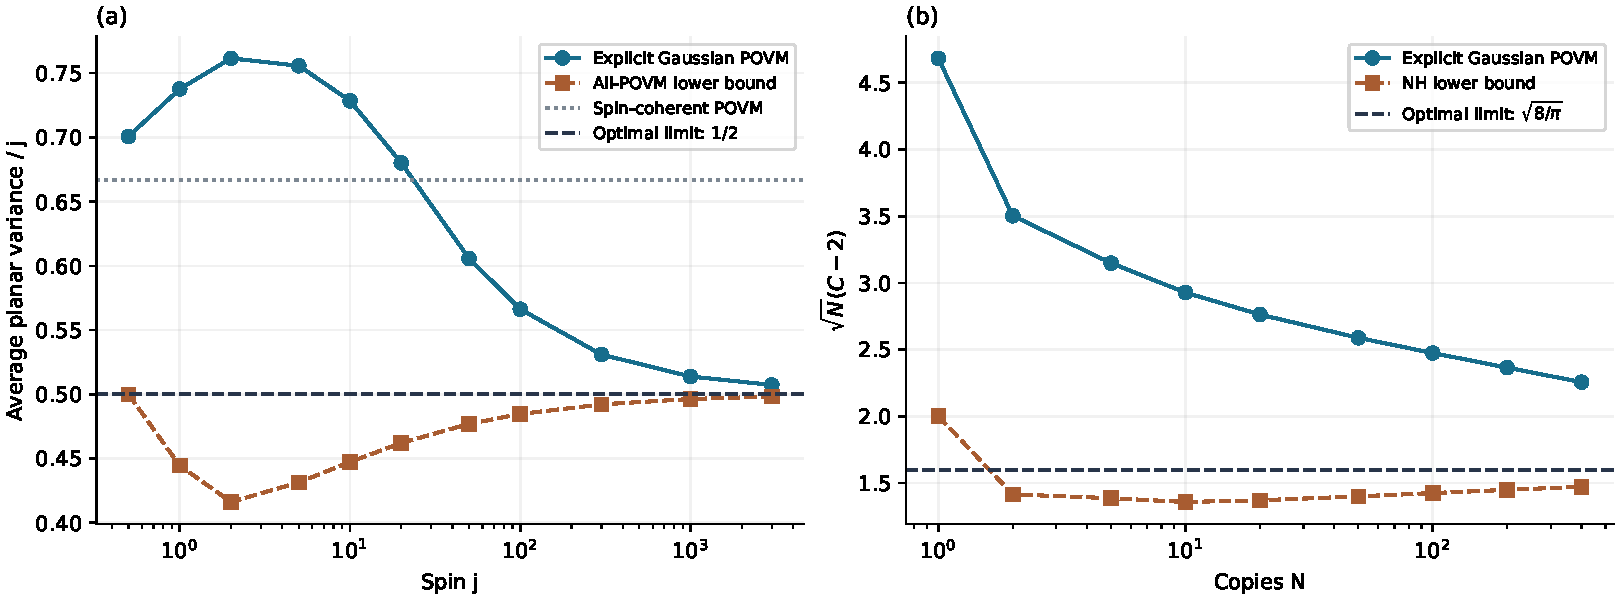
\includegraphics[width=\textwidth]{precision_scaling.pdf}
 \caption{\scalingcaption}
 \label{fig:scaling}
\end{figure*}


\section{Discussion}\label{sec:discussion}

The essential constraint is the average population of the measurement
seeds. Local squeezing specifies low-variance states, whereas a valid
measurement also requires their effects to sum to the identity. Column
normalization imposes this condition exactly and leaves the width
available to control the variance. The regularization near the equator
and the estimates at the poles allow the local squeezing balance to be
used throughout the spin sector. This completes the connection between
the established local description \cite{He2011,Dammeier2015} and the
attainable finite-copy correction.

The strict NH gap expresses the same completeness constraint at finite
size. Seeds that saturate the capped certificate cannot resolve the
identity in sufficiently large spin sectors, as shown in
Appendix~\ref{app:NH}. The Gaussian family satisfies completeness
exactly while its variance differs from the lower bound by only $o(j)$.
Schur averaging makes this an $o(\sqrt N)$ Fisher-information deficit
and an $o(N^{-1/2})$ gap in normalized risk. Thus finite-dimensional
nonattainability of the NH bound is compatible with agreement at the
first correction.

The logarithmic width sequence gives an explicit asymptotically optimal
family, while the finite-$N$ example in Section~\ref{sec:gap} shows that
its convergence can be slow. Optimizing the widths for finite-copy
performance and determining higher-order corrections are natural next
questions. The present result concerns local estimation at the maximally
mixed state; extending the construction to a nonzero reference Bloch
vector requires accounting for the corresponding change in sector
states and probabilities.

\section{Conclusions}\label{sec:conclusions}

The optimal normalized risk for two-parameter qubit estimation at the
maximally mixed state is
$2+\sqrt{8/\pi}\,N^{-1/2}+o(N^{-1/2})$.
An exact Gaussian-column decomposition attains the underlying common
planar variance $j/2+o(j)$, and its score estimator is exactly locally
unbiased for every finite $N$. The matching all-POVM lower bound fixes
the first correction and places the strict finite-copy NH gap at a
smaller asymptotic order.

\section*{Data and code availability}
[DATA AND CODE AVAILABILITY TO BE CONFIRMED]

\begin{acknowledgments}
[ACKNOWLEDGMENTS AND FUNDING TO BE COMPLETED]
\end{acknowledgments}

\section*{Declarations}
[DECLARATIONS TO BE CONFIRMED]

\appendix
\section{Exact statistical reduction and seed representation}
\label{app:reduction}
This appendix proves Lemma~\ref{lem:reduction} and establishes
the seed representation used in the lower bound.
\begin{proof}
The global reference state and tangents are $I/2^N$ and
$2J_a^{\mathrm{tot}}/2^N$. They are block diagonal in
\eqref{eq:schur} and scalar on each multiplicity space. For an
arbitrary effect $M_z$, define
$E_{z|j}=\nu_j^{-1}\tr_{\mathrm{mult}}(\Pi_jM_z\Pi_j)$.
Discarding the label $j$ reproduces the original local probabilities
and derivatives. Keeping it is a statistical refinement and increases
Fisher information in positive semidefinite order by
Cauchy--Schwarz. Conversely, any conditional POVM lifts to
$E_{z|j}\otimes I_{\nu_j}$. Since $\dot P_{N,j}=0$, its Fisher matrix
is the weighted sum of the conditional matrices.

For any measurement, let $u(z)=\nabla\log p_\theta(z)|_0$ and
$F=\E_0[uu^{\mathsf T}]$. When $F$ is invertible, the estimator
$F^{-1}u$ satisfies \eqref{eq:unbiased} and has covariance $F^{-1}$.
For every locally unbiased estimator,
\[
 \E_0\bigl[(\widehat\theta-F^{-1}u)
 (\widehat\theta-F^{-1}u)^{\mathsf T}\bigr]
 =\Cov_0(\widehat\theta)-F^{-1}\succeq0.
\]
If $F$ is singular, the identity
$\E_0[\widehat\theta u^{\mathsf T}]=I_2$ is impossible.
Full rank of the reference state ensures that these score identities
also apply to continuous outcomes, using the scalar trace measure as
a dominating measure. In particular the scores are bounded.
For positive definite $F$, $\tr F^{-1}\geq4/\tr F$.
Randomizing the measurement by rotations about $z$ and retaining the
rotation label gives $F=(\tr F/2)I_2$ without changing its trace.
This proves the first two assertions.

Refining effects to rank one cannot decrease Fisher information.
A pure state decomposition of $I/d$ corresponds to the effects
$E_a=dp_a\ket{\psi_a}\bra{\psi_a}$. Its probability is $p_a$ and its
score is $2(\ip{J_x}_{\psi_a},\ip{J_y}_{\psi_a})$. Completeness fixes
\[
 \sum_a p_a\ip{J_x^2+J_y^2}_{\psi_a}
 =\frac1d\tr(J_x^2+J_y^2)=\frac23j(j+1).
\]
Subtracting the average variance gives the last identity.
\end{proof}

For use in the lower bound, we give a real nonnegative seed form. In
the $J_z$ basis, indexed by $m=-j,\ldots,j$, set
\begin{equation}
\begin{aligned}
c_m&=\sqrt{(j-m)(j+m+1)},\qquad
n_a=\sum_m v_{a,m}^2,\\
h_a&=\sum_{m=-j}^{j-1}c_mv_{a,m}v_{a,m+1}.
\end{aligned}
\label{eq:seeds}
\end{equation}
Then
\begin{equation}
 T_j=\frac4d\max_{v_a\geq0,\;\sum_a v_{a,m}^2=1}
 \sum_a\frac{h_a^2}{n_a}.
 \label{eq:seed-opt}
\end{equation}
Indeed, for a complex rank-one vector $w$ its trace contribution is
$4|\bra wJ_+\ket w|^2/(d\norm w^2)$. Replacing each coordinate by
its modulus increases this quantity and preserves diagonal
populations. Completeness is then restored exactly by the phase
orbit
\begin{equation}
\begin{aligned}
E_{a\ell}&=\frac1L\ket{v_{a\ell}}\bra{v_{a\ell}},\qquad
v_{a\ell,m}=v_{a,m}e^{-im\phi_\ell},\\
\phi_\ell&=\frac{2\pi\ell}{L},\qquad L\geq\max(d,3).
\end{aligned}
\label{eq:phase-orbit}
\end{equation}
All nonzero frequencies $m-m'$ have absolute value below $L$, and
their phase averages vanish. The first and second phase moments give
zero score mean and an isotropic Fisher matrix. This argument also
covers half-integer spins, since $m-m'$ is always an integer.

The maximum in \eqref{eq:seed-opt} is attained. To see this, put
$p_{a,m}=v_{a,m}^2/n_a$ and $\mu_a=n_a/d$. These define a probability
measure on the compact probability simplex with mean
$(1/d,\ldots,1/d)$. Its objective is the integral of the continuous
function $4(\sum_mc_m\sqrt{p_mp_{m+1}})^2$. Weak compactness gives
an optimizer. A supporting affine function for its concave envelope
at the uniform vector, followed by Carath\'eodory's theorem on the
contact set, reduces the support to at most $d$ seeds. We will use
attainment only when discussing strict finite-dimensional gaps.


\section{A sum-of-squares lower bound}\label{sec:lower}
This appendix establishes the all-POVM lower bound used in
Theorem~\ref{thm:main} and defines the capped quantities entering
the NH value in Section~\ref{sec:gap}.
Index the $d$ nodes by $i=0,\ldots,d-1$ and the
$d-1$ edges by $i=0,\ldots,d-2$. Thus
$c_i=\sqrt{(i+1)(d-1-i)}$. For $j>0$, let $\tau_j$ be the unique
positive solution of
\begin{equation}
 \sum_{i=0}^{d-2}(c_i-\tau_j)_+=\tau_j.
 \label{eq:cap}
\end{equation}
Write
\begin{equation}
\begin{aligned}
a_i&=\min(c_i,\tau_j),\qquad S_j=\sum_i c_i a_i,\\
D_j&=\sum_i c_i^2-S_j,\qquad L_j=\frac{D_j}{d}.
\end{aligned}
\label{eq:cap-quantities}
\end{equation}
Set all four quantities to zero when $j=0$.

\begin{proposition}\label{prop:lower}
For every spin, $V_j\geq L_j$. Moreover,
\begin{equation}
 L_j=\frac j2+o(j),\qquad 0\leq L_j\leq\frac j2+\frac14.
 \label{eq:lower-asymptotic}
\end{equation}
\end{proposition}
\begin{proof}
The left side of \eqref{eq:cap} minus its right side is continuous
and strictly decreasing, positive at zero and negative at
$\max_i c_i$. Define
\[
 r_0=0,\qquad r_{i+1}-r_i=c_i/a_i-1.
\]
Equation~\eqref{eq:cap} gives $r_{d-1}=1$ and $0\leq r_i\leq1$.
Put $a_{-1}=a_{d-1}=0$ and
$\lambda_i=(1-r_{i-1})a_{i-1}^2+r_{i+1}a_i^2$, omitting absent
boundary terms. If $K$ has off-diagonal entries $K_{i,i+1}=c_i$,
direct expansion gives, for every real $v$ and $t$,
\begin{equation}
\begin{aligned}
&v^{\mathsf T}(\diag\lambda+t^2I-tK)v\\
&\quad=\sum_{i=0}^{d-1}\bigl[(1-r_i)(tv_i-a_iv_{i+1})^2\\
&\qquad\qquad{}+r_i(tv_i-a_{i-1}v_{i-1})^2\bigr]\geq0.
\end{aligned}
\label{eq:sos}
\end{equation}
Here absent vector components are zero, and
$a_i(1-r_i+r_{i+1})=c_i$. Also $\sum_i\lambda_i=S_j$.
For a nonzero seed take $t=h_a/n_a$ in \eqref{eq:sos}. Then
$h_a^2/n_a\leq\sum_i\lambda_i v_{a,i}^2$.
Summing over the complete seed family yields $T_j\leq4S_j/d$.
Since $\sum_i c_i^2=\frac23j(j+1)d$,
Lemma~\ref{lem:reduction} proves $V_j\geq D_j/d$.
Thus \eqref{eq:sos} is itself a certificate for the entire POVM
optimization.

For the asymptotic statement let $J=j+1/2=d/2$. Then
$c_i^2=J^2-(i+1-J)^2$ and $\tau_j<J$. The cap equation implies
\begin{equation}
 \tau_j^2\leq D_j=\sum_i c_i(c_i-\tau_j)_+
 \leq J\tau_j\leq J^2.
 \label{eq:cap-squeeze}
\end{equation}
If $\tau_j\leq(1-\eta)J$ on an unbounded subsequence for some
$\eta>0$, a fixed positive fraction of the central edges satisfy
$c_i\geq(1-\eta/2)J$. Their contribution to
$\sum_i(c_i-\tau_j)_+$ is of order $J^2$, contradicting
\eqref{eq:cap}. Hence $\tau_j/J\to1$ and $D_j/J^2\to1$.
Dividing \eqref{eq:cap-squeeze} by $d=2J$ proves both claims.
\end{proof}


\section{Global Gaussian energy estimates}\label{sec:energy-proof}
This appendix proves the Gaussian variance upper bound used in
Theorem~\ref{thm:main}. The denominator in \eqref{eq:W} couples all
columns; a lower bound on $h^2/s$ separates them into energies
that can be estimated uniformly. Set
\begin{equation}
\begin{aligned}
q(t)&=\sqrt{(J^2-t^2)_+},\qquad B_m=\sqrt{J^2-m^2},\\
k_m&=\frac{c_{m-1}+c_m}{2},
\end{aligned}
\label{eq:q}
\end{equation}
where $c_{-j-1}=c_j=0$. From $h^2/s\geq2qh-q^2s$,
\begin{equation}
\begin{aligned}
W_j[b]&\leq U_j[b]\\
&:=\frac1d\int_\R
\left[\sum_m(A_m+q^2)v_m^2-2qh_j\right]dt\\
&=\frac1d\left(\sum_m I_m+\sum_{m=-j}^{j-1}G_m+\sum_m R_m\right),
\end{aligned}
\label{eq:energy}
\end{equation}
where every term is nonnegative:
\begin{equation}
\begin{aligned}
I_m&=\int_\R(k_m-q(t))^2v_m(t)^2dt,\\
G_m&=c_m\int_\R q(t)(v_{m+1}(t)-v_m(t))^2dt,\\
R_m&=\frac{(c_m-c_{m-1})^2}{4}.
\end{aligned}
\label{eq:energies}
\end{equation}
To verify the second equality in \eqref{eq:energy}, use
\begin{align*}
 h_j&=\sum_m k_mv_m^2-\frac12\sum_m c_m(v_{m+1}-v_m)^2,\\
 A_m-k_m^2&=R_m.
\end{align*}

\begin{theorem}\label{thm:energy}
For every fixed positive $b\in C^2([-1,1])$,
\begin{equation}
 \lim_{j\to\infty}\frac{U_j[b]}j
 =\frac12\int_{-1}^1
 \left(x^2b(x)+\frac1{4b(x)}\right)dx.
 \label{eq:functional}
\end{equation}
For $b_\epsilon(x)=(2\sqrt{x^2+\epsilon^2})^{-1}$ and the explicit
sequence \eqref{eq:epsilon},
\begin{equation}
 \frac{U_j[b_{\epsilon_j}]}j\longrightarrow\frac12,
 \qquad W_j[b_{\epsilon_j}]=\frac j2+o(j).
 \label{eq:explicit-energy}
\end{equation}
\end{theorem}

\subsection{Uniform control at the poles}

All constants denoted $C_b$ in this subsection depend only on a
positive lower bound for $b$ and an upper bound for its $C^2$ norm.
For $r(s)=J-|s|\geq1/2$,
\begin{equation}
\begin{aligned}
Jr(s)&\leq B(s)^2:=J^2-s^2\leq2Jr(s),\\
S(s)&\asymp_b r(s),\qquad |S'(s)|\leq C_b,\\
|S''(s)|&\leq C_b/J.
\end{aligned}
\label{eq:pole-scales}
\end{equation}
The positive-part map is 1-Lipschitz. Therefore, for every real $t$,
including $|t|\geq J$,
\begin{equation}
 |q(t)-B_m|\leq\frac{|t^2-m^2|}{B_m}.
 \label{eq:global-q}
\end{equation}
Under $v_m(t)^2dt$, $t-m$ is normal with variance $S_m=S(m)$.
Taking its second and fourth moments gives
\begin{equation}
 \int(q-B_m)^2v_m^2dt
 \leq\frac{4m^2S_m+3S_m^2}{B_m^2}\leq C_bJ.
 \label{eq:position-bound}
\end{equation}
Since $c_m=q(m+1/2)$, the same inequality gives
$|k_m-B_m|^2\leq CJ/r(m)$. Consequently, for every column,
\begin{equation}
 0\leq I_m\leq C_bJ.
 \label{eq:I-bound}
\end{equation}

For the gradient term write $Y=(t-s)/\sqrt{S(s)}$. Direct
differentiation yields
\begin{equation}
 \partial_sv_s=v_s\left[\frac{Y}{2\sqrt S}
 +\frac{S'}{4S}(Y^2-1)\right].
 \label{eq:derivative}
\end{equation}
The square-root H\"older inequality and \eqref{eq:pole-scales}
imply
\begin{align}
 q(s+\sqrt S Y)
 &\leq B(s)+\sqrt{2J\sqrt S|Y|+SY^2}\notag\\
 &\leq C_b\sqrt{Jr(s)}(1+|Y|).
 \label{eq:q-bound}
\end{align}
This bound also includes all tails crossing the poles. Gaussian
moments in \eqref{eq:derivative} now give
\begin{equation}
\begin{aligned}
&\int q(t)(\partial_sv_s(t))^2dt\\
&\quad\leq C_b\sqrt{Jr(s)}
\left(\frac1{S(s)}+\frac{S'(s)^2}{S(s)^2}\right)\\
&\quad\leq C_b\sqrt{\frac J{r(s)}}.
\end{aligned}
\label{eq:derivative-bound}
\end{equation}
For $s\in[m,m+1]$, $c_m\leq C\sqrt{Jr(s)}$. Integral
Cauchy--Schwarz in $s$ therefore yields
\begin{equation}
\begin{aligned}
0\leq G_m
&\leq c_m\int_m^{m+1}\int q(t)(\partial_sv_s(t))^2dt\,ds\\
&\leq C_bJ.
\end{aligned}
\label{eq:G-bound}
\end{equation}
Finally $R_m\leq CJ/r(m)$, whence
\begin{equation}
 \frac1d\sum_mR_m=O(\log(2+J))=o(J).
 \label{eq:R-bound}
\end{equation}
For fixed $0<\delta<1$, the columns with
$|m|>(1-\delta)J$ and their incident edges thus contribute at most
$C_b(\delta+J^{-1})$ to $U_j[b]/J$.

\subsection{The interior limit}

Fix $\delta>0$ and restrict to $x_m=m/J$ with
$|x_m|\leq1-\delta$. All errors below are uniform over this set;
constants may depend on $b$ and $\delta$. Put
$f(x)=\sqrt{1-x^2}$. Centered expansion gives
$k_m-B_m=O_\delta(J^{-1})$. A global remainder estimate is
\begin{equation}
\begin{aligned}
&\left|q(m+z)-B_m+\frac{m}{B_m}z\right|\\
&\quad\leq\left(\frac1{2B_m}+\frac{4m^2}{B_m^3}\right)z^2
             +\frac{z^4}{B_m^3}.
\end{aligned}
\label{eq:q-taylor}
\end{equation}
This follows from
$|\sqrt{u_+}-B-(u-B^2)/(2B)|\leq(u-B^2)^2/(2B^3)$,
valid for every real $u$ and $B>0$, by taking
$u=J^2-(m+z)^2$. Thus the estimate also covers the region where
$q$ vanishes. Set $z=\sqrt{Ja(x_m)}Y$. Its right-hand side is
$O_{b,\delta}(Y^2+J^{-1}Y^4)$. Squaring and using the Gaussian
moments through order eight gives
\begin{equation}
\begin{aligned}
\frac{I_m}{J}
 &=a(x_m)f'(x_m)^2+O_{b,\delta}(J^{-1/2})\\
 &=x_m^2b(x_m)+O_{b,\delta}(J^{-1/2}).
\end{aligned}
\label{eq:I-limit}
\end{equation}

For the gradient term, use the weighted norm
$\norm w_q^2=\int q(t)|w(t)|^2dt$. In an interior unit interval,
$S\asymp_{b,\delta}J$, $S'=O_b(1)$, and $S''=O_b(J^{-1})$.
Equation~\eqref{eq:derivative} and one further derivative imply
\begin{equation}
\begin{aligned}
\norm{\partial_sv_s}_q&=O_{b,\delta}(1),\\
\norm{\partial_s^2v_s}_q&=O_{b,\delta}(J^{-1/2}).
\end{aligned}
\label{eq:H2}
\end{equation}
Indeed, $\partial_s^2v_s/v_s$ is a polynomial in $Y$ of degree at
most four, with coefficients $O_{b,\delta}(J^{-1})$, and $q\leq J$.
Two applications of the fundamental theorem of calculus and
Minkowski's inequality give
\begin{equation}
\begin{aligned}
&\norm{v_{m+1}-v_m-\partial_mv_m}_q\\
&\quad\leq\int_m^{m+1}\int_m^s
\norm{\partial_u^2v_u}_qdu\,ds\\
&\quad=O_{b,\delta}(J^{-1/2}).
\end{aligned}
\label{eq:finite-diff}
\end{equation}
Thus the squared norm of $v_{m+1}-v_m$ differs from that of
$\partial_mv_m$ by $O_{b,\delta}(J^{-1/2})$.
In \eqref{eq:derivative}, the squared translation term contributes
\begin{align*}
 &\frac1{4Ja(x_m)}\E\bigl[q(m+\sqrt{Ja(x_m)}Y)Y^2\bigr]\\
 &\qquad=\frac{f(x_m)}{4a(x_m)}+O_{b,\delta}(J^{-1/2}).
\end{align*}
The cross term containing $S'$ is $O_{b,\delta}(J^{-1/2})$ and its
square is $O_{b,\delta}(J^{-1})$. Since
$c_m/J=f(x_m)+O_\delta(J^{-1})$, we obtain
\begin{equation}
 \frac{G_m}{J}=\frac1{4b(x_m)}+O_{b,\delta}(J^{-1/2}).
 \label{eq:G-limit}
\end{equation}
The Riemann sums in \eqref{eq:I-limit} and \eqref{eq:G-limit},
divided by $d=2J$, give the integral in \eqref{eq:functional} over
the interior. Equations~\eqref{eq:I-bound}, \eqref{eq:G-bound}, and
\eqref{eq:R-bound} allow $\delta\downarrow0$ after $j\to\infty$.
This proves \eqref{eq:functional}, since $J/j\to1$.

\subsection{One explicit width sequence}

Pointwise minimization of the integrand in \eqref{eq:functional}
suggests $b_*(x)=1/(2|x|)$ away from the equator. Use instead
\begin{equation}
\begin{aligned}
b_\epsilon(x)&=\frac1{2\sqrt{x^2+\epsilon^2}},\\
a_\epsilon(x)&=\frac{1-x^2}{2\sqrt{x^2+\epsilon^2}},
\qquad 0<\epsilon\leq1.
\end{aligned}
\label{eq:regularized-width}
\end{equation}
An exact integral evaluates the limiting functional:
\begin{equation}
 \frac12\int_{-1}^1\left(x^2b_\epsilon+\frac1{4b_\epsilon}\right)dx
 =\frac12\sqrt{1+\epsilon^2}.
 \label{eq:integral}
\end{equation}
For fixed $\epsilon$ this already implies
$\limsup_jV_j/j\leq\sqrt{1+\epsilon^2}/2$. Together with
Proposition~\ref{prop:lower}, it proves \eqref{eq:roof-asymptotic}.
To specify a single attaining family, we retain the parameter
dependence of the estimates above.

There is an absolute constant $C>0$ such that whenever
$0<\delta<1/2$, $J\geq\epsilon^{-1}$, and $J\delta\geq1$,
\begin{equation}
\begin{aligned}
&\left|\frac{U_j[b_\epsilon]}J-\frac12\sqrt{1+\epsilon^2}\right|\\
&\quad\leq C\epsilon^{-7}(\delta+J^{-1})\\
&\qquad{}+C(\epsilon^{-2}\delta^{-6}
             +\epsilon^{-12}\delta^{-4})J^{-1/2}
       +C\frac{1+\log(2J)}J.
\end{aligned}
\label{eq:uniform-error}
\end{equation}
We give explicit bounds supporting these exponents. The formulas
in \eqref{eq:regularized-width} give
\begin{equation}
\begin{aligned}
\frac1{2\sqrt2}&\leq b_\epsilon\leq\frac1{2\epsilon},\\
\norm{a_\epsilon'}_\infty&\leq C\epsilon^{-3},\qquad
\norm{a_\epsilon''}_\infty\leq C\epsilon^{-5}.
\end{aligned}
\label{eq:parameter-bounds}
\end{equation}
Equation~\eqref{eq:position-bound} then gives
$I_m\leq C\epsilon^{-2}J$. In \eqref{eq:q-bound} one may take the
constant $C\epsilon^{-1/2}$. Using $S\geq cr$ and
$|S'|\leq C\epsilon^{-3}$ in \eqref{eq:derivative-bound} gives
$G_m\leq C\epsilon^{-7}J$. The deleted pole regions therefore
produce the first term of \eqref{eq:uniform-error}; the corresponding
integral tails are at most $C\epsilon^{-1}\delta$.

In the interior, $S\geq cJ\delta$, $S\leq CJ\epsilon^{-1}$,
and $S',JS''$ have the polynomial bounds \eqref{eq:parameter-bounds}.
To check all derivative constants, write the bracket in
\eqref{eq:derivative} as
$g=A Y+B(Y^2-1)$, where $A=(2\sqrt S)^{-1}$ and $B=S'/(4S)$.
Then $\partial_s^2v_s/v_s=g^2+\partial_sg$, and
\begin{align*}
 \partial_sY&=-S^{-1/2}-\frac{S'}{2S}Y,\qquad
 A'=-\frac{S'}{4S^{3/2}},\\
 B'&=\frac{S''}{4S}-\frac{S'^2}{4S^2}.
\end{align*}
The four types of coefficient in $\partial_s^2v_s/v_s$ are
$S^{-1}$, $S'/S^{3/2}$, $S''/S$, and $S'^2/S^2$. Hence, using
$q\leq J$ and fixed Gaussian moments,
\begin{equation}
\begin{aligned}
\norm{\partial_sv_s}_q&\leq C\epsilon^{-3}\delta^{-1},\\
\norm{\partial_s^2v_s}_q&\leq C\epsilon^{-6}\delta^{-2}J^{-1/2}.
\end{aligned}
\label{eq:explicit-H2}
\end{equation}
The finite-difference replacement therefore changes the squared
norm by at most $C\epsilon^{-12}\delta^{-4}J^{-1/2}$.
For the position term, use the global remainder
\eqref{eq:q-taylor}, $S\leq CJ\epsilon^{-1}$,
$B_m\geq J\sqrt\delta$, and
$|k_m-B_m|\leq CJ^{-1}\delta^{-3/2}$.
Gaussian moments through order eight give the uniform bound
\begin{equation}
 \left|I_m/J-x_m^2b_\epsilon(x_m)\right|
 \leq C\epsilon^{-2}\delta^{-6}J^{-1/2}.
 \label{eq:explicit-I}
\end{equation}
For the gradient expectation one can use the global bound
\eqref{eq:global-q} directly:
\begin{align*}
 &|q(m+\sqrt S Y)-B_m|\\
 &\quad\leq C\left[\sqrt J\epsilon^{-1/2}\delta^{-1/2}|Y|
             +\epsilon^{-1}\delta^{-1/2}Y^2\right].
\end{align*}
The errors in the squared translation term, the cross term with
$S'$, and its square are at most
$C\epsilon^{-1}\delta^{-2}J^{-1/2}$,
$C\epsilon^{-3}\delta^{-2}J^{-1/2}$, and
$C\epsilon^{-6}\delta^{-2}J^{-1}$, respectively. Including
\eqref{eq:explicit-H2} and the change from $c_m/J$ to $f(x_m)$,
\begin{equation}
 \left|G_m/J-1/(4b_\epsilon(x_m))\right|
 \leq C\epsilon^{-12}\delta^{-4}J^{-1/2}.
 \label{eq:explicit-G}
\end{equation}
Finally the derivative of $x^2b_\epsilon+1/(4b_\epsilon)$ has
absolute value at most $3/2$, uniformly in $\epsilon$.
This controls the Riemann-sum error. These
are all terms in the preceding argument and prove
\eqref{eq:uniform-error}.

Now use \eqref{eq:epsilon} and, only in the proof, take
$\delta_j=\epsilon_j^8$. The pole error is
$O(1/\log J)+O((\log J)^7/J)$. The interior error is
$O((\log J)^{50}/\sqrt J)$.
Every term tends to zero. Therefore
$U_j[b_{\epsilon_j}]/j\to1/2$.
Since $L_j\leq V_j\leq W_j[b_{\epsilon_j}]\leq
U_j[b_{\epsilon_j}]$, \eqref{eq:explicit-energy} follows.
The cutoff $\delta_j$ has no role in the measurement; all columns
and all real outcomes $t$ remain present.


\section{Schur averaging and completion of the main proof}\label{sec:averaging}
This appendix completes Theorem~\ref{thm:main} by averaging the spin
bounds over the Schur probabilities. Write $\E_N$ for expectation under
$P_{N,j}$. The following moment identities and remainder estimate control
the sum as the number of sectors grows.

\begin{lemma}\label{lem:averaging}
The Schur probabilities satisfy
\begin{equation}
\begin{aligned}
\E_N[j(j+1)]&=\frac{3N}{4},\\
\frac{\E_Nj}{\sqrt N}&\longrightarrow\sqrt{\frac2\pi}.
\end{aligned}
\label{eq:schur-moments}
\end{equation}
If a fixed sequence $r_j$, defined on all nonnegative integer and
half-integer spins, has finite entries and $r_j=o(j)$, then
$\E_Nr_j=o(\sqrt N)$.
\end{lemma}
\begin{proof}
The first identity is the trace of
$(J_x^{\mathrm{tot}})^2+(J_y^{\mathrm{tot}})^2+
(J_z^{\mathrm{tot}})^2$ in $I/2^N$.
Let $S_N$ be a sum of $N$ independent symmetric signs. Summation
by parts in
$P_{N,j}=(2j+1)(q_j-q_{j+1})$,
$q_j=2^{-N}\binom N{N/2-j}$, gives the exact identity
\begin{equation}
 \E_Nj=\E|S_N|-\frac12+\frac12\Pr(S_N=0).
 \label{eq:walk}
\end{equation}
The binomial sums are
\[
 \E|S_{2n}|=2n\frac{\binom{2n}n}{2^{2n}},\qquad
 \E|S_{2n+1}|=(2n+1)\frac{\binom{2n}n}{2^{2n}}.
\]
Stirling's formula proves \eqref{eq:schur-moments} for both parities.
For any $\eta>0$, choose a fixed $K_\eta$ such that
$|r_j|\leq\eta j$ when $j\geq K_\eta$. If
$M_\eta=\max_{j<K_\eta}|r_j|$, then
\[
 \frac{\E_N|r_j|}{\sqrt N}
 \leq\eta\frac{\E_Nj}{\sqrt N}+\frac{M_\eta}{\sqrt N}.
\]
Letting first $N\to\infty$ and then $\eta\downarrow0$ proves the
claim. In particular, finitely many small-spin values cause no
problem.
\end{proof}

By Theorem~\ref{thm:energy} and Lemma~\ref{lem:averaging},
\begin{equation}
 \E_N W_j^{\g}=\frac12\sqrt{\frac2\pi}\sqrt N+o(\sqrt N).
 \label{eq:averaged-W}
\end{equation}
The same conclusion holds with $W_j^{\g}$ replaced by either
$V_j$ or $L_j$. For any of these three sequences $Z_j$,
\begin{equation}
\begin{aligned}
\frac{4N}{2N-4\E_NZ_j}
 &=2+\frac{4\E_NZ_j}{N}+o(N^{-1/2})\\
 &=2+\sqrt{\frac8\pi}N^{-1/2}+o(N^{-1/2}).
\end{aligned}
\label{eq:risk-expansion}
\end{equation}
The lower bound holds for every POVM by
Proposition~\ref{prop:lower}, and the explicit family supplies the
matching upper bound. This completes the proof of
Theorem~\ref{thm:main}.


\section{The NH formula and strict finite-copy separation}\label{app:NH}
Here we supply the finite-dimensional facts used in
Section~\ref{sec:gap}. The two-parameter NH bound can be expressed
as a convex first-moment optimization, or equivalently as its usual
semidefinite relaxation \cite{HayashiOuyang2023,ZhangHayashi2026}.
Put $D=2^N$ and $Z=X+iY$ for arbitrary Hermitian first moments.
Eliminating the auxiliary operator blocks gives the objective
\[
\begin{aligned}
\mathcal F(Z)
 &=\min_{W\succeq Z^\dagger Z,\;W\succeq ZZ^\dagger}\tr W\\
 &=\tr Z^\dagger Z+
   \max_{0\preceq R\preceq I}\tr R(ZZ^\dagger-Z^\dagger Z).
\end{aligned}
\]
The equality follows by taking the positive spectral part of
$ZZ^\dagger-Z^\dagger Z$. The normalized NH risk is $(N/D)$ times
the minimum of $\mathcal F$ under the first-moment constraints.

Use the Schur basis with each multiplicity label retained, and let
$R$ be diagonal with the entries $r_i$ from Appendix~\ref{sec:lower}
on each spin block. Then
\[
 \mathcal F(Z)\geq
 \sum_{\alpha,\beta}(1+r_\alpha-r_\beta)|Z_{\alpha\beta}|^2.
\]
Every coefficient is nonnegative. On a raising edge it is
$1-r_i+r_{i+1}=c_i/a_i$. The unbiasedness constraints imply
$\sum_{\text{raising edges}}c_i\operatorname{Re}Z_{i+1,i}=D$.
Thus Cauchy--Schwarz on these edges gives
$\mathcal F(Z)\geq D^2/S_{\mathrm{tot}}$, where
$S_{\mathrm{tot}}=\sum_j\nu_jS_j$. This bound applies to all complex
$Z$, including entries connecting different spin blocks.

To attain it, take adjacent raising matrices in each sector with
real nonnegative entries $x_{j,i}$, identical on the multiplicity
space. Set $w_j=P_{N,j}/d$. Their objective before multiplication
by $N$ is
\begin{equation}
\begin{aligned}
&\sum_jw_j f_j(x_j),\\
f_j(x)&=\sum_i x_i^2+\frac12\sum_{i=0}^{d-1}|x_i^2-x_{i-1}^2|\\
&=\sum_{i=0}^{d-1}\max(x_{i-1}^2,x_i^2).
\end{aligned}
\label{eq:NH-objective}
\end{equation}
where $x_{-1}=x_{d-1}=0$. The zero means and cross derivatives vanish;
the remaining unbiasedness constraint is
$\sum_jw_j\sum_i c_ix_{j,i}=1$.
Expressions containing $S_j^{-1}$ below include only $j>0$ sectors;
the $j=0$ sector contributes zero.
With $r_i$ defined in Appendix~\ref{sec:lower},
\begin{equation}
\begin{aligned}
f_j(x)&\geq\sum_i(1-r_i+r_{i+1})x_i^2\\
&=\sum_i\frac{c_i}{a_i}x_i^2
\geq\frac{(\sum_i c_ix_i)^2}{S_j}.
\end{aligned}
\label{eq:NH-CS}
\end{equation}
The first inequality supports each maximum by a convex combination
of its two entries. At $x_i=a_i$, it is an equality: $r_i$ selects
the larger entry on each uncapped tail and mixes only two equal
entries on the plateau. The second inequality is Cauchy--Schwarz
and is also an equality there. A further weighted
Cauchy--Schwarz inequality across sectors proves that the minimum
is $1/\sum_jw_jS_j$, achieved by
$x_{j,i}=a_{j,i}/\sum_kw_kS_k$. Multiplication by $N$ proves
\eqref{eq:NH}.

Suppose now that the seed maximum \eqref{eq:seed-opt} attains the
upper bound $4S_j/d$. Every seed then saturates the nonnegative
terms of \eqref{eq:sos} with $t=h/n\geq0$.
For $t>0$, the kernel recurrence and connectedness force every
coordinate of a nonzero seed to be positive. An edge with $c_i>
\tau_j$ has $r_{i+1}>0$ and $1-r_i>0$, so the two adjacent
equations force $t=\tau_j$. All such seeds are therefore multiples
of a single vector $u$. Its plateau coordinates can be set to one,
and on the left tail
\begin{equation}
 u_i=(a_i/\tau_j)u_{i+1};
 \label{eq:tail-recursion}
\end{equation}
the right tail is its reflection. For $t=0$, the matrix in
\eqref{eq:sos} is diagonal and only its two endpoint entries can
vanish; all interior $\lambda_i$ are strictly positive.

If $c_1<\tau_j$, the first two edges on the left are uncapped.
Equation~\eqref{eq:tail-recursion} then forces every positive-$t$
seed to satisfy $v_1=(c_1/\tau_j)v_2$, while every zero-$t$ seed
vanishes at both nodes. Hence the sum of their effects obeys
$M_{11}=(c_1/\tau_j)^2M_{22}$, which is incompatible with
$M=I$. Attainment of the seed maximum makes the resulting
inequality strict.

To verify $c_1<\tau_j$ for all $j\geq5$, set $n=2j\geq10$.
At $n=10$ the six central edges give
\begin{align*}
 \sum_i(c_i-c_1)_+
 &=2(\sqrt{24}+\sqrt{28}+\sqrt{30})-6\sqrt{18}\\
 &>\sqrt{18}=c_1.
\end{align*}
For a fully rational check, the three ratios to $\sqrt{18}$
exceed respectively $23/20$, $6/5$, and $5/4$; twice their
sum minus six exceeds one. For each fixed $i\geq2$,
\[
 \frac{c_i}{c_1}=
 \sqrt{\frac{(i+1)(n-i)}{2(n-1)}}
\]
increases with $n$. The three edges $i=2,3,4$ and their three
reflections remain distinct for $n\geq10$. Thus
$\sum_i(c_i-c_1)_+>c_1$ for every such $n$, and the monotonicity
of \eqref{eq:cap} implies $\tau_j>c_1$.
For $N\geq10$ the largest-spin sector $j=N/2$ has positive
probability and a strict Fisher deficit, proving
$C_N>C_N^{\nh}$.

% 由 REVTeX 自动选择 apsrev4-2，并保留文章题目控制项。
\bibliography{references}
\end{document}


